\documentclass[11pt]{article}

\input{$HOME/imajin/preamble.tex}

\begin{document}

\fancyhf{}
\fancyhead[R]{Matthew Jin (mjin2002)}
\setlength{\headheight}{14pt}
\pagestyle{fancy}

\centerline{\Large CS 149: Programming Assignment 1}
\centerline{Autumn 2024-25}

\section{Parallel Fractal Generation Using Threads}

\begin{figure}[hpt]
  \centering
  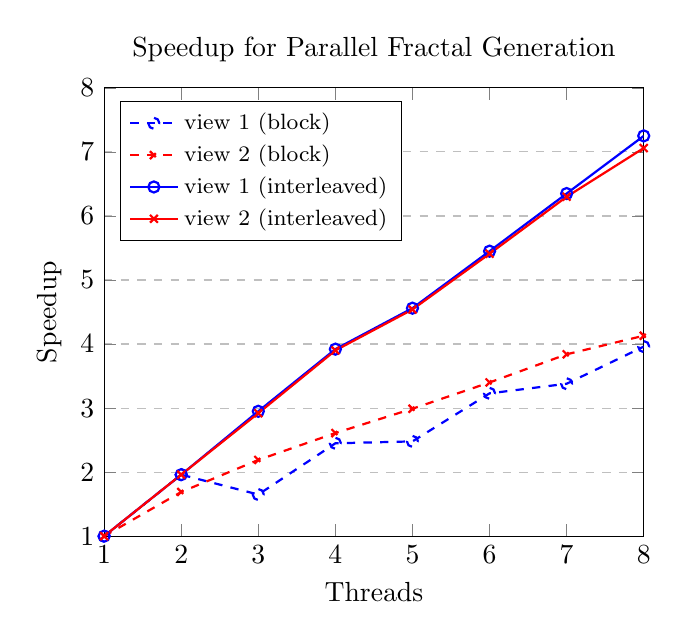
\begin{tikzpicture}
    \begin{axis}[
      title={Speedup for Parallel Fractal Generation},
      xlabel={Threads},
      ylabel={Speedup},
      xmin=1, xmax=8,
      ymin=1, ymax=8,
      ytick={1,2,3,4,5,6,7,8},
      ymajorgrids=true,
      grid style=dashed,
      legend pos=north west,
      legend style={font=\footnotesize},
      legend cell align={left},
      ]
    \addplot[
      thick,
      color=blue,
      mark=o,
      style=dashed,
      ]
      coordinates {
        (1,1.00)(2,1.96)(3,1.65)(4,2.45)(5,2.48)(6,3.23)(7,3.38)(8,3.96)
      };
    \addplot[
      thick,
      color=red,
      mark=x,
      style=dashed,
      ]
      coordinates {
        (1,1.00)(2,1.69)(3,2.19)(4,2.61)(5,2.99)(6,3.40)(7,3.84)(8,4.13)
      };
    \addplot[
      thick,
      color=blue,
      mark=o,
      ]
      coordinates {
        (1,1.00)(2,1.96)(3,2.95)(4,3.92)(5,4.56)(6,5.45)(7,6.35)(8,7.25)
      };
    \addplot[
      thick,
      color=red,
      mark=x,
      ]
      coordinates {
        (1,1.00)(2,1.96)(3,2.92)(4,3.90)(5,4.54)(6,5.41)(7,6.30)(8,7.06)
      };
    \legend{view 1 (block),view 2 (block),view 1 (interleaved),view 2 (interleaved)}
    \end{axis}
  \end{tikzpicture}
  \caption{Dashed lines are the speedup of the spatial decomposition (block)
  image partitioning method. Solid lines are the interleaved partitioning method
  with \ttt{rowsPer=3}.}
  \label{fig:speedup}
\end{figure}

The spatial decomposition fractal generation method exhibits less than linear speedup due
to the fact that certain pixels of the Mandelbrot set image take longer to
compute. This may be because certain points need to iterate up to
\ttt{maxIterations} before the program can determine if the pixel should be
black or white, significantly slowing down the thread's computation.

\smallskip
Observing the 3-thread case (and others) for view 1, we see that the thread
assigned to the middle rows of the image takes much longer than the others,
indicating that determining whether a point was in the Mandelbrot set did indeed
take more computation. This explains the slower speedup shown in the graph as
the thread(s) assigned to the middle part the image (the section with the most
white pixels) will end up taking a greater fraction of time than the other
threads.

\smallskip
To resolve this issue, we switch from the spatial decomposition (block) method
for partitioning the image to an interleaved method where each thread computes
\ttt{rowsPer} rows at a time, spaced based on the number of threads.
Technically, this is a generalization of the first method, as setting
\ttt{rowsPer=height/numThreads} would cause each thread to take their respective
``block" of the image. However, to distribute the number of rows that are
majority white pixels more evenly among the threads, we choose \ttt{rowsPer=3},
giving us the solid lines in Figure \ref{fig:speedup}.

\smallskip
Running the improved code with 16 threads instead of 8 provides no performance
benefits at all, and sometimes even results in a worse speedup. This is because
the myth machines only support up to 8 threads running concurrently. Thus,
adding more will not result in more parallel computation and instead slows the
program down by introducing more context switching overhead.

\medskip
Note that for the interleaved method, there is a slightly larger slowdown
moving from 4 to 5 threads. Perhaps this is because 4 threads can be distributed
with one thread per core? Then, the 5th thread would put two threads on one core
which could contribute to the noticeable drop in speedup.

\section{Vectorizing Code Using SIMD Intrinsics}

\begin{figure}[hpt]
  \centering
  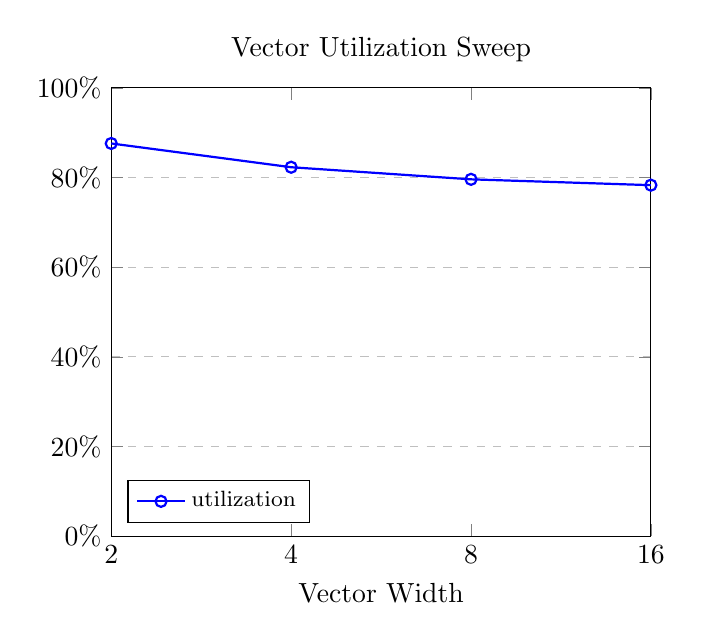
\begin{tikzpicture}
    \begin{semilogxaxis}[
      title={Vector Utilization Sweep},
      xlabel={Vector Width},
      xmin=2, xmax=16,
      ymin=0, ymax=100,
      xtick={2,4,8,16},
      xticklabels={2,4,8,16},
      yticklabel={$\pgfmathprintnumber{\tick}\%$},
      ymajorgrids=true,
      grid style=dashed,
      legend pos=south west,
      legend style={font=\footnotesize},
      legend cell align={left},
      ]
    \addplot[
      thick,
      color=blue,
      mark=o,
      ]
      coordinates {
        (2,87.6)(4,82.3)(8,79.6)(16,78.3)
      };
    \legend{utilization}
    \end{semilogxaxis}
  \end{tikzpicture}
  \caption{Vector utilization trend for vector widths 2, 4, 8, and 16.}
  \label{fig:vecutil}
\end{figure}

Vector utilization decreases as the vector width increases because wider vectors
are more likely to encounter the case where a single element needs to continue
computation while the rest of the lanes are inactive. 

\smallskip
As an extreme example, take the exponent vector $\begin{bmatrix} 1 & 1 & 1 & 10
& 1 & 1 & 1 & 1 \end{bmatrix}$. For vector width 2, each pair of elements would
be at 100\% utilization except the second which needs to iterate and multiply 10
times at 50\% utilization. For vector width 8, the entire group of 8 elements
needs to iterate 10 times at 12.5\% utilization. Hence, increasing the vector
width would decrease vector utilization.

\section{Parallel Fractal Generation Using ISPC}

\subsection{A Few ISPC Basics}

Since we are using 8-wide AVX2 instructions, each operation is
computed across 8 datapoints at a time. Thus, we should expect the maximum total
speed up to be $8 \times 8 = 64$. However, running the ISPC program only gives
us a speed up of 5.05 for view 1. Since checking whether a pixel is in the
Mandelbrot set or not is done in groups of 8, an imbalance in the number of
iterations it takes for each pixel to complete its computation would result in
less vector utilization and slower speedup. These issues will be most prevalent
along the boundaries of the image where a single vector might includes both
white and black pixels. This is reflected in view 2 having a slower speedup of
4.29 compared with view 1 as the image has more ``edges."

\subsection{ISPC Tasks}

With 2 tasks, we get a speed up of 9.90 relative to the serial execution and
1.96 relative to the single-thread ISPC execution. The 1.96 speedup tracks with
the speedup we get from moving from one to two threads in Program 1.

\smallskip
The Intel(R) Core(TM) i7-7700K CPU has four two-way multithreaded cores that can
each run two multiply-and-add vector instructions at a time. Putting this all
together, this means the entire CPU can execute $4 \times 2 \times 2 = 16$
vector instructions at a time. Thus, we should launch 16 tasks in parallel which
gives us a speedup of over 32 times. This works best because each CPU's
vector computation resources are fully utilized.

% TODO: extra credit

\section{Iterative \ttt{sqrt}}

The base speedup for a random input is around 4.22 using ISPC and around 31.14
using task ISPC. The speedup due to multicore parallelization is
$\frac{31.14}{4.22} \approx 7.38$.

\smallskip
If we modify the input array to be all 0s, we end up with a 7.43 speedup using
ISPC and 52.99 speedup using task ISPC. The multicore parallelization speed up
is $\frac{52.99}{7.43} \approx 7.13$. Since the input is a constant, the
\ttt{sqrt} algorithm will take the same number of iterations for all inputs, so
the single core speedup is close to 8. However, the multicore speedup decreased
compared to the original input which may be due to the fact that some cores may
lag behind others and other scheduling overheads.

\smallskip
In order to minimize the speedup of ISPC without tasks, we can construct an
input vector taht contains one slow input (i.e. $x=0$) and seven fast inputs
(i.e. $x=1$). Then, the sequential program will run instantly for 7/8 of the
input and spend most of its time processing the interleaved 1/8. Meanwhile, the
every parallel vector spawned by the ISPC program will need processing the slow
input at 1/8 vector utilization. Using this input scheme nets us a single core
ISPC speedup of 0.94. The overhead of processing the vector instructions ends up
making the program slower than the serial version.

% TODO: extra credit

\section{BLAS \ttt{saxpy}}

Running the base \ttt{saxpy} program shows that there is a 1.04x speedup from
using tasks. The reason using multiple cores does not improve the runtime is
because the program is bottlenecked by the memory bandwidth since the
computation can be done quickly. % FIXME: check

% TODO: extra credit(s)

\section{Making \ttt{K-Means} Faster}

We started by measuring the time the program spent in \ttt{computeAssignments},
\ttt{computeCentroids}, and \ttt{computeCost}.

\begin{table}[hpt]
  \centering
  \begin{tabular}{l|l}
    \ttt{computeAssignments} & 6254.47 ms \\
    \hline
    \ttt{computeCentroids} & 958.32 ms \\
    \hline
    \ttt{computeCost} & 1846.52 ms \\
    \hline
    Total Time & 9075.97 ms \\
  \end{tabular}
  \caption{Time spent in each k-means function.}
  \label{tab:times}
\end{table}

We also measured the time spent in \ttt{dists} which ended up slowing down the
entire program to about 12000 ms, of which about half was spent in \ttt{dists}.
However, since \ttt{dists} only loops over \ttt{N=10} while
\ttt{computeAssignments} loops over \ttt{M=1e6}, we decided to optimize
\ttt{computeAssignments} by splitting up the work over \ttt{M}.

\smallskip
First, we move \ttt{minDist} into the main k-means loop as it only needs to be
initialized once since the values independent across iterations. A pointer to
this array is added to the worker arguments so each thread can access it in
\ttt{computeAssignments}. Then, in the main loop, we initialize \ttt{numThreads}
threads and assign each thread a contiguous block of indices across \ttt{M} to
compute. This change leads to a runtime of around 5000ms which corresponds to a
speed up of $\sim\!1.8-1.9$.

\smallskip
To further improve our program, we consider the loop structure in
\ttt{computeAssignments} and how it affects the cache. The outer loop
controls access to the \ttt{clusterCentroids} array which had size $\ttt{K}
\times \ttt{N} = 300$ for \ttt{K=3}. For one iteration of the outer loop, the
inner loop has to iterate over all \ttt{M} indices in the data. Since \ttt{M'}
is large, earlier indices would be pushed out of the cache (128 KiB) by later
indices, only to be loaded back in cache on the second iteration of the outer
loop. These repeated cache misses would slow down the overall runtime of the
program. In order to fix this issue, we can switch the order of the inner and
outer loops. Then, each index in \ttt{M} will only need to sit in the cache once
while the inner loop calculates the distance to all \ttt{K=3} centroids. Once
the distance calculations are complete, that index will never be needed again
and can be safely pushed out of the cache.

\smallskip
This small change, combined with threading, results in a final runtime of
3798.54ms compared to the original 9075.97ms giving us a speedup of 2.4!

\end{document}
